\documentclass[border=1pt]{standalone}
\usepackage{fontspec}
\usepackage[dvipsnames,svgnames]{xcolor} % Extended color support
\usepackage{tikz}
\usepackage{pgfplots}
\usepackage{amsmath}
\usepackage{amssymb}
\usepackage{mathtools}
\usepackage{unicode-math}
\usepackage{graphicx}
\usepackage{microtype}
\usepackage{enumitem}

\pgfplotsset{
  compat=1.18
}

%\setmainfont{Libertinus Sans}
%\setsansfont{Libertinus Sans}
%\setmonofont{Libertinus Mono}
%\setmathfont{Libertinus Math}

\setmainfont{Noto Sans}
\setsansfont{Noto Sans}
\setmonofont{Noto Sans Mono}
\setmathfont[
  Path=fonts/,
  Extension=.ttf
]{NotoSansMath-Regular}

\usetikzlibrary{
  calc,
  positioning,
  intersections,
  through,
  angles,
  quotes,
  arrows.meta,
  patterns,
  decorations.pathreplacing,
  decorations.markings,
  decorations.text,
  shapes,
  shapes.geometric,
  matrix,
  fit,
  backgrounds,
  fadings
}

\begin{document}
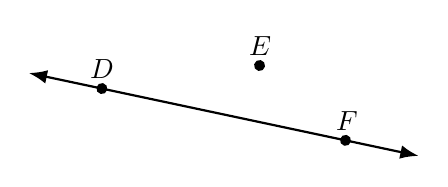
\begin{tikzpicture}[>=Latex]
  \tikzset{
    dimline/.style={
      arrows={Bar[length=0pt,width=14pt]}-{Bar[length=0pt,width=14pt]}
    },
    dot ends/.style={
      {Circle[length=2pt]}-{Circle[length=2pt]}
    },
    %    every path/.style={thick},
    % every node/.style={font=\large}
  }

  \begin{scope}[rotate=-12]
    \coordinate (a) at (0,0);
    \coordinate (c) at (90pt,0);
    \coordinate (b) at ($(a)!0.6!(c)+(0,20pt)$);
    \draw[thick, <->] ($(a)!-0.3!(c)$)--($(a)!1.3!(c)$);

    \fill[] (a) circle (2pt) node[above] {$D$};
    \fill[] (c) circle (2pt) node[above] {$F$};
    \fill[] (b) circle (2pt) node[above] {$E$};

  \end{scope}

\end{tikzpicture}

\end{document}
